\chapter{Estado del arte}\label{estadoarte}

En este capítulo se describirán los fundamentos teóricos y tecnológicos del proyecto. En primer lugar se presentará 
la identificación de tráfico y las distintas técnicas que existen para ello. También se explicará Bro \cite{broindex}, el 
sistema de monitorización de tráfico que se usará para 
llevar a cabo el desarrollo del proyecto. Así, se explicará su funcionamiento y, especialmente, el lenguaje de programación 
incorporado, analizándose cómo gestiona los eventos y sus funcionalidades básicas, así como la posibilidad de ampliar estas.

\intro Por último, se presentará de forma teórica en que consiste el emparejamiento de flujos y de qué forma 
se podría usar para identificar el tráfico.

\section{Identificación de tráfico}

Una definición de identificación de tráfico podría ser la siguiente, ``la clasificación del tráfico implica la atribución de objetos 
de tráfico a las clases de tráfico que los generan. La identificación usa terminología similar a la clasificación de tráfico. El 
término identificación se suele usar cuando se realiza de forma granular." cita de \cite{khalife2014}.

\intro Esta técnica es usada para realizar muchas tareas de gestión y seguridad de la red. Como por ejemplo medidas de seguridad, 
aseguramiento de calidad de servicio \cite{microqos} e ingeniería de tráfico \cite{khalife2016}.

\subsection{Técnicas de identificación de tráfico}

La identificación de tráfico se puede realizar en tres niveles distintos, dependiendo de la granularidad que se aplique 
\cite{khalife2016}.

\begin{itemize}
\item Paquetes. Se realiza el análisis a los paquetes de forma individual.
\item Flujos. Se analizan los flujos a partir de ciertos parámetros.
\item Host. Se identifican las aplicaciones que usan los distintos equipos de la red.
\end{itemize}

\intro La más usada es la identificación basada en flujos, que es la que se usará en este trabajo.

\subsection{Identificación de tráfico basada en flujos}

En esta técnica, los flujos se analizan individualmente, ya sea un análisis global de la conexión o de algunos de los paquetes que lo 
componen.

\intro Existen tres técnicas básicas de identificación de tráfico basada en flujos.

\begin{itemize}
\item Por los puertos de la capa de transporte, establecido por \textit{IANA} \cite{iana}.
\item Por el contenido del paquete o \textit{DPI} \cite{payload}.
\item Por la aplicación de técnicas de aprendizaje automático sobre estadísticas de tráfico, \textit{machine learning} \cite{learning}.
\end{itemize}

\subsubsection{Identificación basada en puertos}

Esta técnica se basa en identificar el tráfico dependiendo de los puertos de la capa de transporte, según la asignación estándar 
de IANA \cite{ianaexplicacion}. 

\intro Por lo tanto, IANA es quien asigna el número de puerto oficial a los distintos protocolos, haciendo que, a priori, pueda 
identificar el tráfico por el número de puerto del servidor. 

\intro Esta técnica es la más simple y funcionaba correctamente, pero actualmente no es la más fiable. Esto se debe a la ofuscación de 
puertos, la multiplexación de puertos por diferentes servicios y el uso de otros puertos no oficiales.

\intro Un ejemplo de multiplexación de puertos sería el siguiente. En la actualidad, se están desarrollando multitud de aplicaciones 
web. Estas aplicaciones se conectan mediante el puerto 80, es decir, mediante el protocolo HTTP. Pero esto es solo teoría, pues se 
puede hacer que cualquier aplicación envíe información por el puerto 80, sin que sea HTTP, lo cual daría como resultado una mala 
identificación.

\subsubsection{Aprendizaje automático}

En esta técnica de identificación, se hace uso de clasificadores basados en algoritmos de aprendizaje automático \cite{learning}. Se 
trata de un campo de investigación muy activo actualmente. En estas investigaciones se han propuesto y evaluado múltiples sistemas 
basados en distintos tipos de clasificadores, como redes neuronales, redes bayesianas o lógica fuzzy.

\intro A pesar de ser un campo de investigación muy vivo y en el cual los métodos implementados son cada vez más inteligentes, los 
resultados no son buenos. Son costosos computacionalmente y al necesitar tiempo para el aprendizaje, se dan muchos errores en la 
clasificación.

\subsubsection{DPI}

La Inspección Profunda de Paquetes, DPI por sus siglas en inglés, \textit{Deep Packet Inspection}, realiza un análisis de los 
paquetes, más allá de la cabecera, en busca de cadenas que permitan identificar de manera inequívoca el protocolo \cite{payload}. 
Dichas cadenas podrían ser \textit{GET} o \textit{POST} para el protocolo \textit{HTTP}, por ejemplo.

\intro Esta técnica suele ser usada por los proveedores de servicios de Internet, ISP, \textit{Internet Service Provider} y grandes 
empresas. Se puede decir que es una técnica que no respeta la privacidad, pues analiza la información contenida en el paquete. Aunque 
en el caso de una gran empresa si puede hacerse, pues si se está en la red propia no es delito mirar la información que contienen los 
paquetes.

\intro Esta técnica es la más efectiva en la actualidad, con una buena tasa de identificación y pocos errores \cite{dpiaproximacion}, 
pero presenta problemas a nivel de escalabilidad, al tener que analizar todos los paquetes de forma individual, y de privacidad, al 
entrar dentro de los paquetes, pudiendo llegar a ser ilegal en algunos países.

\section{BRO}

Bro \cite{broindex}, es un analizador de tráfico de red de código abierto, por lo que puede ser usado por quien lo desee 
sin necesidad de pagar licencias. Funciona sobre sistemas basados en Linux y 
Mac OS X. Una de sus principales características es la gran cantidad de información que puede extraer con un solo 
escaneo. Otros monitores de red proporcionan menos información, teniendo que ser el propio administrador el que 
analice después la información obtenida por estos. Por lo tanto, tardará más en resolver los posibles problemas 
que encuentre en la red.

\begin{figure}[H]
  
\includegraphics[width=0.25\textwidth]{imagenes/logo-bro.png}
  \centering
  \caption{Logo de Bro.}
\end{figure}

\intro No tiene interfaz gráfica, por lo que su gestión se realiza desde la línea de comandos. Cuando se analiza 
tráfico, Bro generará unos registros con la información obtenida, los cuales están divididos en función de parámetros definidos por 
parte del equipo que lo ha desarrollado.

\intro Bro incorpora la posibilidad de introducir funcionalidades nuevas, mediante la programación en su 
propio lenguaje de \textit{scripting}, del mismo nombre. Esto se expondrá más adelante y, en el capítulo \ref{implementacion}, se 
mostrará cómo se desarrolla y algunos ejemplos de código escrito en Bro.

\intro El lenguaje de \textit{scripting} está orientado a trabajar con eventos. Por lo tanto, a la hora de añadir una nueva 
funcionalidad habrá que crearla a partir del uso de los eventos que puede gestionar el programa.

\intro \noindent Bro está estructurado de forma que todos los flujos de paquetes que analiza son procesados por el motor de eventos, 
como se puede ver en la Figura \ref{fig.arquitec}. Este motor convierte los flujos de paquetes en procesos de alto nivel, de forma que 
es más sencillo trabajar con ellos. Una vez que estos son tratados se generan los registros correspondientes, los cuales 
podrán ser analizados posteriormente \cite{broarquitectura}.

\begin{figure}[H]
  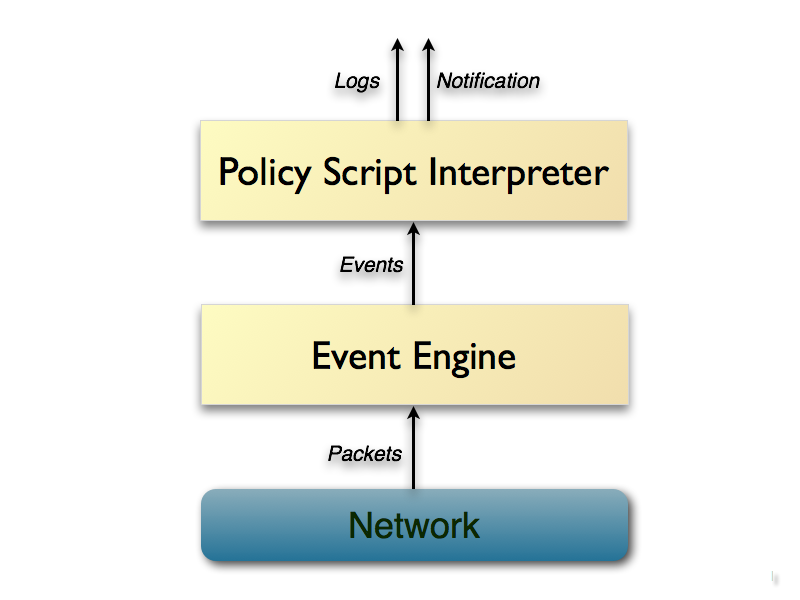
\includegraphics[width=0.7\textwidth]{imagenes/arquitectura-bro.png}
  \centering
  \caption{Arquitectura de Bro.}\label{fig.arquitec}
\end{figure}

\subsection{Funcionalidades básicas de BRO}

La funcionalidad básica de Bro es la monitorización de la red en la que se ejecuta. 
Mientras que se encuentra en ejecución, genera registros o \textit{logs} en texto plano que se 
podrán leer usando un editor de texto. Si se analiza un archivo \textit{pcap} los \textit{logs} no cambiarán tras finalizar el 
procesamiento. Sin embargo, si se analiza tráfico en tiempo real, los registros se irán actualizando a medida que pase el tiempo. 
Algunos de los \textit{logs} que se generarán son los siguientes.

\begin{itemize}
\item \textit{dpd.log}. Consiste en un resumen de los protocolos encontrados en puertos que no son estándar.
\item \textit{dns.log}. Contendrá toda la actividad correspondiente al \textit{DNS}
\item \textit{ftp.log}. Un registro de la actividad a nivel de sesión de \textit{FTP}.
\item \textit{files.log}. Un resumen con los archivos transferidos a través de una red. Incluye 
protocolos \textit{HTTP, FTP y SMTP.}
\item \textit{http.log}. Registro de toda la actividad \textit{HTTP} con sus respuestas.
\item \textit{ssl.log}. Un registro de las sesiones \textit{SSL}, incluidos los certificados que se utilizan.
\item \textit{weird.log}. En este \textit{log} se guarda la información correspondiente a actividad 
inesperada o rara a nivel de protocolo. Al analizar gran cantidad de tráfico no es muy útil, pues normalmente considera un volumen 
importante del tráfico como inesperado, pero a pequeña escala es bastante interesante para detectar, por ejemplo, intrusiones.
\item \textit{conn.log}. Aquí se puede ver la información correspondiente a sesiones \textit{TCP, UDP e ICMP}.
\end{itemize}

\intro Se puede consultar más información sobre \textit{logs} generados por una monitorización de Bro en \cite{brologs}.

\intro Bro dispone además de varios \textit{frameworks} que extienden su funcionalidad. Con ellos se podrán crear \textit{scripts} muy potentes. Algunas de las utilidades más relevantes de estos \textit{frameworks} son las siguientes.
\begin{itemize}
\item \textit{Geolocalización}. Se podrá encontrar la localización geográfica de una IP.
\item \textit{Análisis de ficheros}. El monitor de red tiene la capacidad de trabajar con ficheros.
\item \textit{Framework de loggins}. Con este \textit{framework} se podrá extender los archivos de registro que se generan.
\item \textit{NetControl}. Este \textit{framework} permitirá a Bro conectarse con distintos dispositivos de la red, como 
\textit{switches} o cortafuegos \cite{bronetcontrol}. En la Figura \ref{fig.netcontrol} se puede ver su arquitectura.
\begin{figure}[H]
  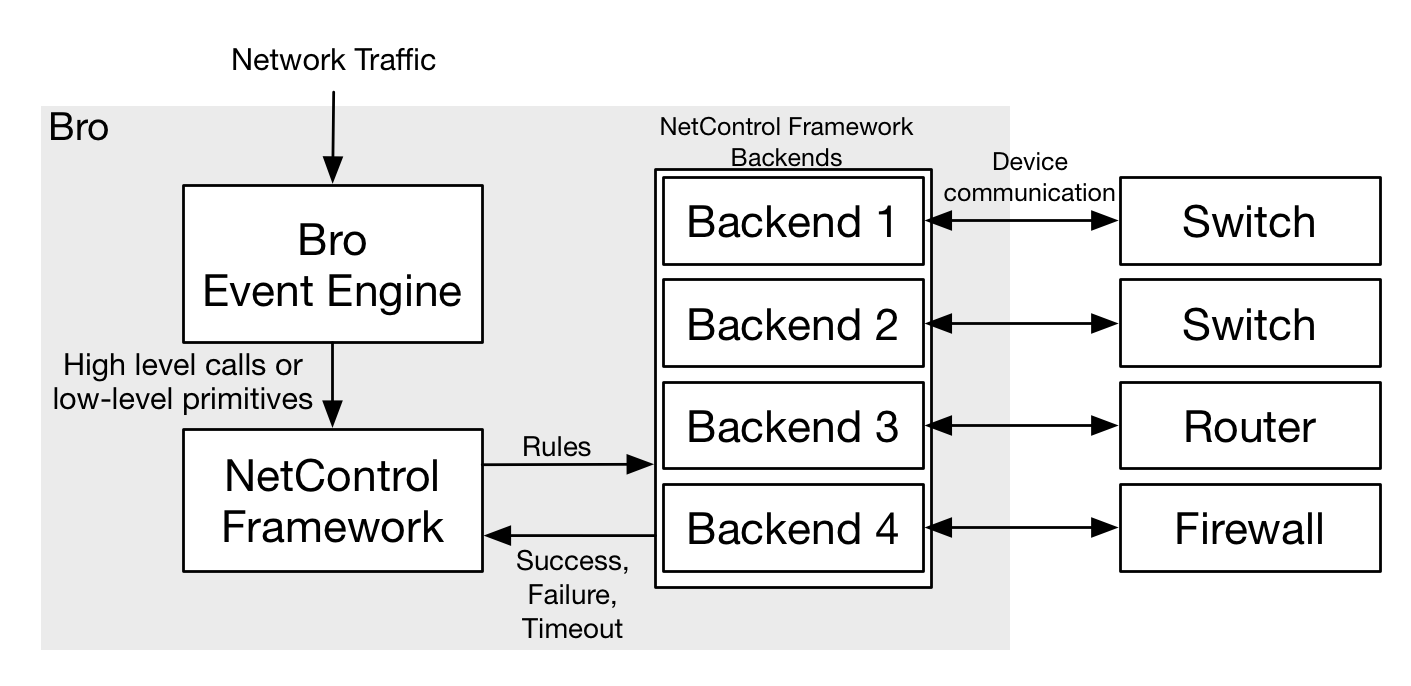
\includegraphics[width=0.7\textwidth]{imagenes/netcarquitectura.png}
  \centering
  \caption{Arquitectura de NetControl.}\label{fig.netcontrol}
\end{figure}
\end{itemize}


\intro Se pueden ver más detalles de estos \textit{frameworks} y otros en \cite{broframeworks}.

\intro A partir de la información de los registros, el administrador del sistema podrá determinar, entre otras cuestiones, si existen 
amenazas en la red o si hay algún componente defectuoso. Para ello deberá hacer uso de los eventos con los que Bro trabaja, para 
obtener un mejor conocimiento de todo el trabajo que se realice sobre la red.

\subsection{Eventos y trazas}
Eventos
que son
trabajan con trazas
que son
la programación con eventos

Un evento se da cuando Bro detecta una determinada acción, por ejemplo, cuando detecta un paquete de respuesta \textit{UDP}, se 
activará el evento \textit{udp_reply}.

\intro Dentro de cada evento se trabajará con la información que capture ese evento. Si el evento captura información de una conexión 
\textit{TCP}, se tendrá que trabajar con esa información y las distintas variables globales que se hayan definido previamente.

\intro Los eventos se activan mediante el tráfico. Una traza es una captura del tráfico de una red. Con casi cualquier programa de 
diagnóstico se puede realizar capturas de red. En la propia web de Bro se encuentran algunos archivos de trazas de red, en 
formato \textit{pcap}, de forma que se puedan realizar pruebas sobre ellos sin necesitar realizar una 
traza propia.

\intro En el caso de Bro se podrá generar trazas de red mediante un \textit{script} de \textit{Python}
\cite{brotrace}, el cual se puede descargar desde el repositorio de \textit{GitHub} de Bro. Con dicho script también 
se podrá trabajar sobre la traza, separando el tráfico entrante del saliente, desglosando en distintos registros 
el tipo de tráfico y demás.

\intro Por lo tanto la programación de Bro esta orientada a eventos. Por lo tanto el orden depende de cuando se ejecute un determinado evento en el análisis.


\subsection{Incorporación de funcionalidades}

La incorporación de funcionalidades al monitoreo realizado por Bro es una característica muy llamativa. Gracias 
a esto se podrá realizar un análisis muy personalizado usando un \textit{script} creado por el administrador de redes. De 
esta forma podrá, por ejemplo, filtrar el tráfico de una determinada IP mientras se sigue analizando el tráfico 
de forma normal, con los registros que genera Bro de forma automática. Es una forma muy sencilla de comprobar 
si por ejemplo el servicio que administra está recibiendo demasiadas peticiones desde una misma IP. Lo cual 
sería un indicio de ataque de denegación de servicio.

\intro A la hora de incorporar funcionalidades a Bro se puede hacer todo lo que se desee. Una búsqueda rápida 
por \textit{GitHub} arrojará una gran cantidad de personas que contribuyen con una gran cantidad de nuevas 
funcionalidades \citep{gitbeacon}. Ahora lo ideal sería incorporar un módulo, de forma que si el resto 
de la comunidad lo desea pueda hacer uso de él de una forma sencilla.

\section{Emparejamiento de flujos}

La técnica de emparejamiento de flujos, fue planteada por el departamento de Teoría de la Señal, 
Telemática y Comunicaciones, \textit{TSTC}, de la Universidad de Granada, en el año 2011 \cite{presentacion} \cite{comparacion}. 
%Luego en el año 2013, el departamento realizó pruebas de la técnica de identificación en un entorno de 
%laboratorio \cite{comparacion}.

\intro En el emparejamiento de flujos, la idea de la que se parte es muy sencilla. Si dos paquetes comparten 
IP's de origen y destino, y puertos de origen y destino, se podrá decir que esos dos paquetes pertenecen a 
la misma clase. Una vez que están identificados como pertenecientes a la misma clase, lo que se debe de hacer 
es comparar los tiempos de esos paquetes, de forma que sean coherentes en el flujo. Si son muy lejanos en el 
tiempo, se podrá descartar que pertenezcan al mismo flujo. Esta idea se puede ver en \cite{comparacion} de una 
forma mucho más técnica.

\intro En el mismo artículo \cite{comparacion} se encuentra la fórmula que se sigue para el emparejamiento.

\begin{equation*}
	F(x,y)=
 	\begin{cases}
	  G(x,y), & NIP(x,y) \geq 1 \\
	  -\infty, & \text{en otro caso}
	 \end{cases}
\end{equation*}

\intro Donde tenemos que G(x,y) se corresponde con la siguiente función:

\begin{displaymath}
G(x,y) = |NIP(x,y) – 1| + 1 / (dp1(x,y) + k1) + 1 / (dp2(x,y) + k1) + 1 / (dt(x,y) + k2)
\end{displaymath}

\intro Las variables de la función son las siguientes: 

\begin{itemize}
\item \textit{x}: Primer paquete a comparar.
\item \textit{y}: Segundo paquete a comparar.
\item \textit{NIP(x,y)}: Es el número de paquetes analizados con las mismas características.
\item \textit{dp1(x,y)}: Se corresponde con los puertos de origen de los dos paquetes.
\item \textit{dp2(x,y)}: Serán los puertos de destino de los dos paquetes.
\item \textit{k1}: Es una variable definida previamente.
\item \textit{k2}: Es otra variable definida antes del comienzo del análisis. En trabajos anteriores esta variable 
y la anterior suelen estar definidas entre 1 y 10000.
\item \textit{dt}: Es la diferencia de tiempo existente entre los tiempos de inicio de los 
paquetes o \textit{timestamps}.
\end{itemize}

\intro Con esta fórmula se obtendrá como resultado un número, el cual será comparado con un umbral que se 
define previamente. Si el umbral definido es pequeño tendremos más flujos emparejados. Si el umbral es mayor 
serán menos los flujos que serán emparejados al no cumplir los requisitos.

\intro El emparejamiento de flujos, por si mismo, sólo identifica el tráfico. Por lo tanto se 
necesitará otra técnica para clasificar el tráfico.
